\section{Suchalgorithmen}
\label{sec:module.Suchalgorithmen}

\subsection{Pfadsuche}
\label{sec:module.Suchalgorithmen.Pfadsuche}
Wir haben drei m�gliche Pfadalgorithmen in unserem Code eingebaut. Via PathFinder-Klasse kann f�r die Pfadsuche der Algorithmus ausgew�hlt werden.


\subsubsection{Simple Algorithmus}
\label{subsec:module.Suchalgorithmen.Pfadsuche.Simple}

Der Simple Algorithmus versucht das Ziel zu erreichen indem er zuerst die eine, dann die andere Achse abl�uft. Sobald ein Hindernis in den Weg kommt, bricht der Algorithmus ab. In der Abbildung \ref{fig:SimplePath} sucht der Algorithmus zuerst den Vertikal-Horizontal Pfad. Da dieser Pfad wegen dem Wasserhindernis (blau) nicht ans Ziel f�hrt, wird via Horizontal-Vertikal Pfad gesucht. Hier wird ein Pfad gefunden. Dieser Algorithmus ist, wie der Name bereits aussagt, sehr einfach aufgebaut und kostet wenig Rechenzeit. Daf�r kann er keinen Hindernissen ausweichen.

\begin{figure}[bth]
\centering

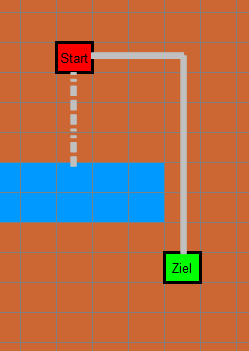
\includegraphics[height=50mm]{91_bilder/simplepath}
\caption{Simple-Path Algorithmus}
\label{fig:SimplePath}
\end{figure}

\subsubsection{A* Algorithmus}
\label{subsec:module.Suchalgorithmen.Pfadsuche.Astar}
Beim A* Algorithmus werden f�r jeden expandierten Knoten die gesch�tzten Kosten f(x) f�r die gesamte Pfadl�nge berechnet. f(x) besteht aus einem Teil g(x) welches die effektiven Kosten vom Startknoten zum aktuellen Knoten berechnet. Der andere Teil h(x) ist ein heuristischer Wert, der die Pfadkosten bis zum Zielknoten approximiert. Dieser Wert muss die effektiven Kosten zum Ziel immer untersch�tzen. Dies ist in unserem Spiel dadurch gegeben, dass sich die Ameisen nicht diagonal bewegen k�nnen, wir aber f�r den heuristischen Wert die Luftlinie zum Ziel verwenden. Die Pfadsuche wird immer bei dem Knoten fortgesetzt welcher die kleinsten Kosten f(x) hat.

Die Abbildung \ref{fig:heuristicAstar} zeigt den effektiven Pfad (grau) vom zu expandierenden roten Knoten mit den minimalen Kosten von 10 Pixel. Die Luftlinie (blau) als heuristischer Wert hat aber nur eine L�nge von 7.6 Pixel. Damit erf�llt unsere Heuristik die Anforderungen des Algorithmus.

\begin{figure}[bth]
\centering
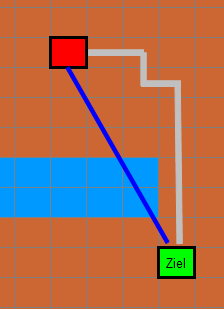
\includegraphics[height=50mm]{91_bilder/heuristicAstar.png}
\caption[A* Pfadsuche]{Heuristische Kosten (blau), Effektive Kosten (grau)}
\label{fig:heuristicAstar}
\end{figure}

Dieser A*-Algorithmus wird in unserem Code f�r eine Pfadsuche �ber alle Pixel (jedes Pixel ist ein Node) verwendet. Der gleiche Code wir aber auch f�r die Pfadsuche mit dem Pfadnetz des HPA* verwendet.

\subsubsection{HPA* Algorthmus}
\label{subsec:module.Suchalgorithmen.Pfadsuche.HPAstar}

Eine Pfadsuche A* �ber alle Pixel ist sehr teuer, da es viel Pfade gibt, die zum Teil nur ein Pixel nebeneinander liegen. Es werden bis zum Schluss verschiedenen Pfaden nachgegangen. Abhilfe zu dieser sehr feinmaschigen Pfadsuche bietet der Hierarchical Pathfinding A* bei welchem im sogenanten Clustering �ber mehrere Pixel verlaufende Kanten und Knoten berechnet werden.

\subsubsubsection{Clustering}
Das Clustering wird w�hrend dem ClusteringTask ausgef�hrt, Dabei wird die Landkarte in sogenannte Clusters unterteilt. Auf dem Bild \ref{fig.clusteredMap} wurde die Karte in 16 Clusters aufgeteilt. 

\begin{figure}[bth]
\centering
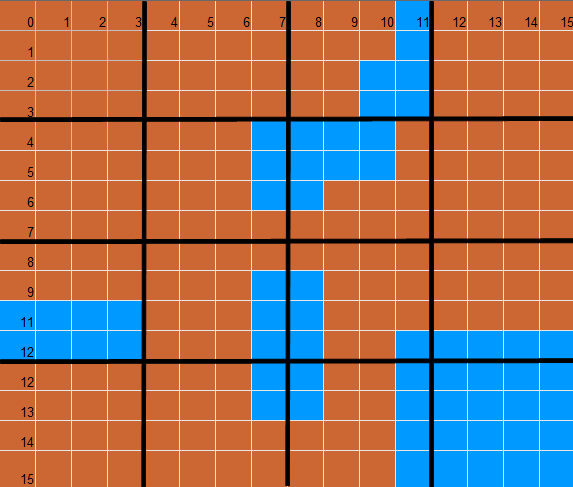
\includegraphics[height=50mm]{91_bilder/clusteredMap.png}
\caption[Clustereinteilung auf der Landkarte.]{Clustereinteilung auf der Landkarte. Clustergr�sse 4x4, Landkarte 16x16}
\label{fig.clusteredMap}
\end{figure}

Danach werden f�r jeden Cluster und einen Nachbar-Cluster aus der Vierer-Nachbarschaft die Verbindungskanten berechnet. Dies kann nat�rlich nur f�r Clusters gemacht werden die auf einem sichtbaren Teil der Landkarte liegen, was zu Begin des Spiel nicht gegeben ist. Deshalb wird der ClusteringTask in jedem Spielzug aufgerufen, in der Hoffnung ein Cluster komplett verbinden zu k�nnen. Sobald eine beliebige Seite eines Clusters berechnet ist, wird diese Aussenkante im Cluster und dem anliegenden Nachbar gespeichert und nicht mehr neu berechnet.

\begin{figure}[bth]
\centering
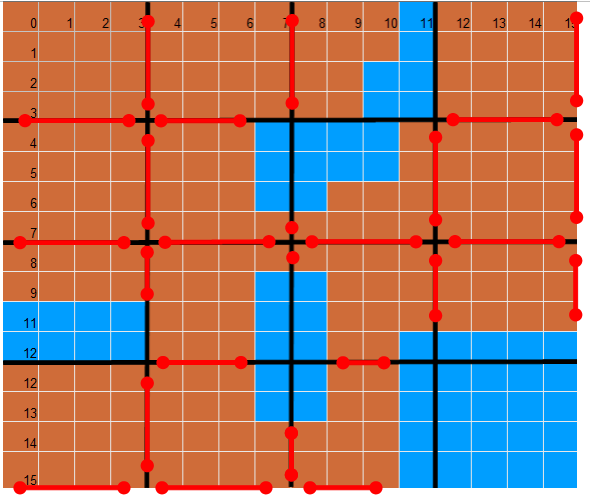
\includegraphics[height=50mm]{91_bilder/clusteredMap2.png}
\caption[Cluster mit berechneten Kanten]{Die Kanten jedes Clusters wurden berechnet}
\label{fig.clusteredMap2}
\end{figure}

Sobald ein Cluster zwei oder mehrere Aussenkanten kennt berechnet er die Innenkanten mit A* welche die Knoten der Aussenkanten verbinden. Dies ergibt nun ein Pfadnetz �ber die Gesamtkarte. Im nachfolgenden Bild sind die Innenkanten (gelb) ersichtlich, die bei den ersten 8 Cluster berechnet wurden.

\begin{figure}[bth]
\centering
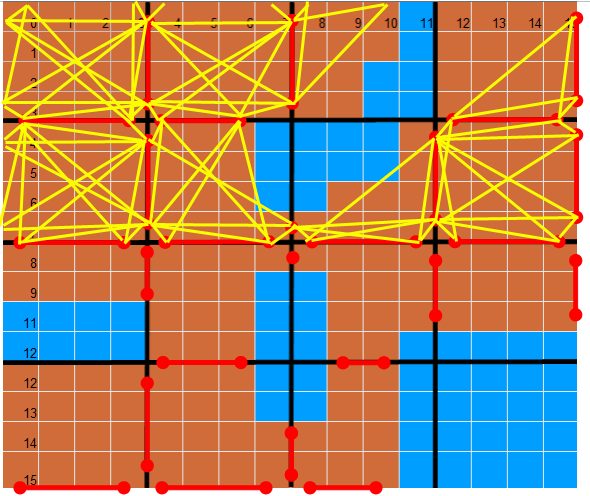
\includegraphics[height=50mm]{91_bilder/clusteredMap3.png}
\caption[Cluster mit Innenkanten]{Darstellung der Innenkanten}
\label{fig.clusteredMap3}
\end{figure}

In der Abbildung \ref{fig.clusteredMap4} wird ein Pfad vom Pixel (3,9) nach (13,9) mittels HPA* gesucht (gr�ne Punkte). Zuerst wird eruiert in welchem Cluster sich das Start- bzw Zielpixel befindet. Danach wird in dem gefundenen Cluster ein Weg zu einem beliebigen Knoten auf der Clusterseite gesucht. Sind diese Knoten erreicht (blaue Pfade), wird nun das vorberechnete Pfadnetz mittels bereits beschrieben A* Algorithmus verwendet um die beiden Knoten auf dem k�rzesten m�glichen Pfad (gelb) zu verbinden.\footnote{Der resultierende Pfad k�nnte mittels Pathsmoothing verk�rzt werden. Dies wurde aber in unserer Arbeit nicht implementiert.}

\begin{figure}[bth]
\centering
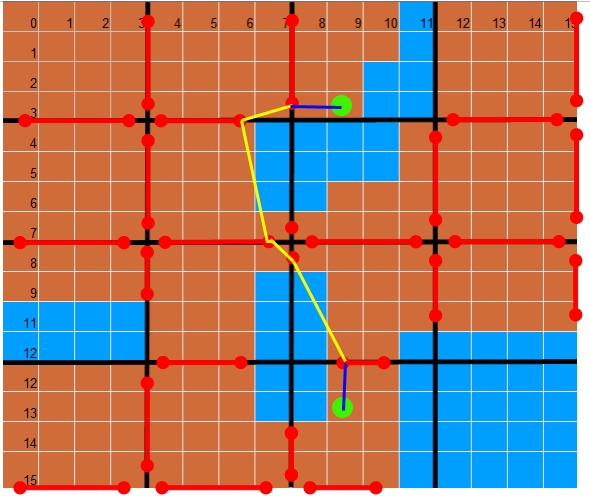
\includegraphics[height=50mm]{91_bilder/clusteredMap4.png}
\caption{Errechneter Weg mittels HPA*}
\label{fig.clusteredMap4}
\end{figure}

\subsubsection{Breitensuche}
\label{subsec:module.Suchalgorithmen.Breitensuche}

Die Breitensuche (engl. breadth-first search (BFS)) war eine der Neuimplementierungen w�hrend der Bachelorarbeit. Man k�nnte die BFS auch f�r die Pfadsuche verwenden, dies w�re aber sehr ineffizient. Wir verwenden diese Suche vielmehr f�r die Umgebung einer Ameise oder eines H�gels zu analysieren. Sie wurde generisch implementierte, so dass sie vielseitig einsetzbar ist. So k�nnen zum Beispiel mittels 'GoalTest' je nach Anwendungsfall die Tiles beschrieben werden welche gesucht sind. Folgende Breitensuche findet die Ameise welche am n�chsten bei einem Food-Tile <r:20,c:16> ist. Sie wird initialisiert indem im Konstruktor die Spielkarte mitgegeben wird, welche durchforscht wird. Zus�tzlich gilt die Einschr�nkung das die Breitensuche nur 40 Tiles durchsuchen darf, was einem Radius von zirka 7 entspricht. Falls keien Ameise gefunden wird gibt der Algorithmus NULL zur�ck.

\begin{verbatim}
AntsBreadthFirstSearch bfs = new AntsBreadthFirstSearch(Ants.getWorld());
Tile food = new Tile(20,16);
Tile antClosestToFood = bfs.findSingleClosestTile(food, 40, new GoalTest() {
      @Override
      public boolean isGoal(Tile tile) {
          return isAntOnTile(tile);
      }
  });
\end{verbatim}

Es ist auch m�glich mehrere Tiles zur�ck zu bekommen. Dazu wird die Methode findClosestTiles(...) aufgerufen.

\newline
\newline

Der gleiche Alogrithmus kann aber auch alle passierbaren Tiles in einem gewissen Umkreis zur�ckgeben. Dies haben wir unteranderem beim Initialisieren der DefendHillMission verwendet. Wir berechnen beim Erstellen der Mission die passierbaren Tiles rundum den H�gel. Runde f�r Runde pr�fen wir diese Tiles auf gegnerische Ameisen um die entsprechenden Verteidigungsmassnahmen zu ergreifen. Der Parameter controlAreaRadius2 definiert den Radius des 'Radars' und kann je nach Profile unterschiedlich eingestellt werden.

\begin{verbatim}
public DefendHillMission(Tile myhill) {
    this.hill = myhill;
    BreadthFirstSearch bfs = new BreadthFirstSearch(Ants.getWorld());
    tilesAroundHill = bfs.floodFill(myhill, controlAreaRadius2);
}
\end{verbatim}